\section{Problem Solution}
\label{sec:solution}

Shown in Figure~\ref{fig:unfolded}, we show the regular pyramid of
Figure~\ref{fig:problem} unfolded onto the plane in such a manner that the edge
$OQ$ remains glued, while the edges $OR$, $OS$, and $OP$ are unglued. An
arbitrary piecewise straight path $\gamma$ from the vertex $P$ to the midpoint
$T$ is then depicted as the green curve on this figure. The differentiable portions,
$PU$ and $UT$, of this path have lengths $\ell_1$ and $\ell_2$, respectively.

The line $PR$ that connects the vertices $P$ and $R$ is orthogonal to the edge
$OQ$ since the triangle $\triangle POQ$ is equilateral. Let the signed distance
from the intersection $M$ of $PR$ with $OQ$ to the intersection $U$ of our path
$\gamma$ and $OQ$ be given by $x$. In the following, we express the total length
$\ell_1 + \ell_2$ of our curve $\gamma$ as a function of this distance $x$ and
minimize it to arrive at the answer.

\begin{figure}[h]
  \centering
  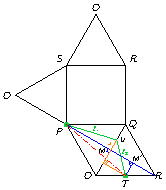
\includegraphics[trim={0 0 0
  0cm},clip,width=0.5\textwidth]{./figures/pyramid-unfolded.pdf}
  \vspace{-8mm}
  \caption{The unfolded regular pyramid.}
  \label{fig:unfolded}
\end{figure}

Since $PM \perp OM$, Pythagoras's theorem yields $\abs{PM} = \sqrt{3}\ell$. By
the same token, $\triangle PMU$ is a right triangle, yielding 
%
\begin{equation}
    \ell_1(x) = \sqrt{x^2 + 3\ell^2}. 
    \label{eq:ell1}
\end{equation}    
%
The perpendicular $TM^\prime$ to $PR$ is parallel to $OQ$ so by the similarity
of the triangles $\triangle OMR$ and $\triangle TM^\prime R$, and the fact that
$\abs{OM} = \ell$, we deduce that $\abs{TM^\prime} = \nicefrac{\ell}{2}$ and
$\abs{MM^\prime} = \nicefrac{\sqrt{3}\ell}{2}$. Using these lengths, along with
$x$, as the side lenghts of the orange right triangle $\triangle T\tilde{M}M$ in
Figure~\ref{fig:unfolded}, we obtain 
%
\begin{equation}
  \ell_2(x) = \sqrt{\ell^2 + \ell x + x^2}.
  \label{eq:ell2}
\end{equation}

The solution that we seek minimizes $\ell_1(x) + \ell_2(x)$. Therefore, we
differentiate this function and set it equal to zero to obtain \[
\frac{2x}{\sqrt{3\ell^2 + x^2}} + \frac{\ell+2x}{\sqrt{\ell^2 + \ell x + x^2}} =
0. \] The solution to this equation is $x^\star = -\nicefrac{\ell}{3}$ as a
simple substitution will show. Plugging this solution into
equations~\eqref{eq:ell1} and~\eqref{eq:ell2} yields \[ \ell_1^\star =
\ell_1(x^\star) = \frac{2\sqrt{7}}{3}\ell, \qquad \ell_2^\star =
\ell_2(x^\star)= \frac{\sqrt{7}}{3}\ell. \] Summing these two optimal values
gives the shortest distance between points $P$ and $T$ on the regular square
pyramid as \[ \ell_1(x^\star) + \ell_2(x^\star) = \sqrt{7}\ell. \]

\begin{lem}
    The (green) path that yields the shortest distance $\sqrt{7}\ell$ is a
    straight line.
\end{lem}

\begin{proof}
    Perhaps the easiest way to show this is to use the law of cosines to show
    that the edge $PT$ of the triangle $\triangle POT$ has length equal to
    $\sqrt{7}\ell$ so that our solution for the green path coincides with the
    dash-dotted red line on Figure~\ref{fig:unfolded}.

    \begin{align*}
        \abs{PT}_{\text{red}}^2 &= (2\ell)^2 + \ell^2 - 2 \cdot 2\ell \cdot \ell
        \cos{120^\circ} = 7\ell^2
    \end{align*}
\end{proof}
